\paragraph{QuizziPedia::Back-End::App::Controllers::SummaryController}
\label{QuizziPedia::Back-End::App::Controllers::SummaryController}
\begin{figure}[ht]
	\centering
	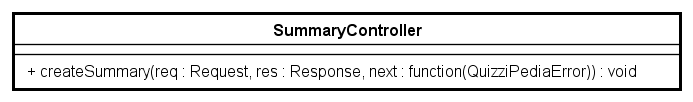
\includegraphics[scale=0.45]{UML/Classi/Back-End/QuizziPedia_Back-End_App_Controllers_SummaryController.png}
	\caption{QuizziPedia::Back-End::App::Controllers::SummaryController}
\end{figure}
\FloatBarrier

\begin{itemize}
	\item \textbf{Descrizione}:
	classe che gestisce la logica applicativa riguardante la visualizzazione e la modifica dei riepiloghi dei questionari.
	\item \textbf{Utilizzo}:
	viene utilizzata per implementare le funzionalità necessarie a gestire le richieste \textit{REST\ped{G}} legate ai riepiloghi dei questionari.
	\item \textbf{Relazione con altre classi}:
	\begin{itemize}
			\item \textbf{IN \texttt{UserRouter}}:
			classe che gestisce le richieste relative alla registrazione, alla gestione della sessione e alla cronologia dei questionari svolti di un utente;
			\item \textbf{OUT \texttt{SummaryModel}}:
			classe che modella i riepiloghi dei questionari.
	\end{itemize}
	\item \textbf{Metodi}:
	\begin{itemize}
		\item \texttt{+ createSummary(req: Request, res: Response, next: \\function(QuizziPediaError))}\\
		Crea un riepilogo.\\
		\textbf{Parametri}:
		\begin{itemize}
			\item \texttt{req: Request}\\
			Rappresenta la richiesta inviata al \textit{server\ped{G}}. Contiene l'identificativo del questionario per cui verrà creato il riepilogo e le risposte date alle domande;
			\item \texttt{res: Response}\\
			Rappresenta la risposta che il \textit{server\ped{G}} fornirà al termine dell'esecuzione del metodo;
			\item \texttt{next: function(QuizziPediaError)}\\
			Rappresenta la \textit{callback\ped{G}} che il metodo deve chiamare al termine dell'elaborazione per passare il controllo ai successivi \textit{middleware\ped{G}}. La presenza del parametro facoltativo \texttt{QuizziPediaError} attiva la catena di gestione dell'errore in sostituzione della normale catena di gestione delle richieste.
		\end{itemize}
	\end{itemize}
\end{itemize}